\documentclass[a4paper, 12pt]{article} 

%--------------------------------------
%Russian-specific packages
%--------------------------------------
%\usepackage[warn]{mathtext}
\usepackage[T2A]{fontenc}
\usepackage[utf8]{inputenc}
\usepackage[english,russian]{babel}
\usepackage[intlimits]{amsmath}
\usepackage{esint}
%--------------------------------------
%Hyphenation rules
%--------------------------------------
\usepackage{hyphenat}
\hyphenation{ма-те-ма-ти-ка вос-ста-нав-ли-вать}
%--------------------------------------
%Packages
%--------------------------------------
\usepackage{amsmath}
\usepackage{amssymb}
\usepackage{amsfonts}
\usepackage{amsthm}
\usepackage{latexsym}
\usepackage{mathtools}
\usepackage{epstopdf}
\usepackage{etoolbox}%Булевые операторы
\usepackage{extsizes}%Выставление произвольного шрифта в \documentclass
\usepackage{geometry}%Разметка листа
\usepackage{indentfirst}
\usepackage{wrapfig}%Создание обтекаемых текстом объектов
\usepackage{fancyhdr}%Создание колонтитулов
\usepackage{setspace}%Настройка интерлиньяжа
\usepackage{lastpage}%Вывод номера последней страницы в документе, \lastpage
\usepackage{soul}%Изменение параметров начертания
\usepackage{hyperref}%Две строчки с настройкой гиперссылок внутри получаеммого
\usepackage[usenames,dvipsnames,svgnames,table,rgb]{xcolor}% pdf-документа
\usepackage{multicol}%Позволяет писать текст в несколько колонок
\usepackage{cite}%Работа с библиографией
\usepackage{subfigure}% Человеческая вставка нескольких картинок
\usepackage{tikz}%Рисование рисунков
\usepackage{float}
% Для картинок Моти
\usepackage{misccorr}
\usepackage{lscape}
\usepackage{cmap}
\usepackage{hyperref}
\usepackage{xcolor}



\usepackage{graphicx,xcolor}
\graphicspath{{Pictures/}}
\DeclareGraphicsExtensions{.pdf,.png,.jpg}

%----------------------------------------
%Список окружений
%----------------------------------------
\newenvironment {theor}[2]
{\smallskip \par \textbf{#1.} \textit{#2}  \par $\blacktriangleleft$}
{\flushright{$\blacktriangleright$} \medskip \par} %лемма/теорема с доказательством
\newenvironment {proofn}
{\par $\blacktriangleleft$}
{$\blacktriangleright$ \par} %доказательство
%----------------------------------------
%Список команд
%----------------------------------------
\newcommand{\grad}
{\mathop{\mathrm{grad}}\nolimits} %градиент

\newcommand{\diver}
{\mathop{\mathrm{div}}\nolimits} %дивергенция

\newcommand{\Def}[1]
{\underline{\textbf{#1}}} %определение

\newcommand{\RN}[1]
{\MakeUppercase{\romannumeral #1}} %римские цифры

\newcommand {\theornp}[2]
{\textbf{#1.} \textit{ #2} \par} %Написание леммы/теоремы без доказательства

\newcommand{\qrq}
{\ensuremath{\quad \Rightarrow \quad}} %Человеческий знак следствия

\newcommand{\qlrq}
{\ensuremath{\quad \Leftrightarrow \quad}} %Человеческий знак равносильности

\renewcommand{\phi}{\varphi} %Нормальный знак фи

\newcommand{\me}
{\ensuremath{\mathbb{E}}}

\newcommand{\md}
{\ensuremath{\mathbb{D}}}




%\renewcommand{\vec}{\overline}




%----------------------------------------
%Разметка листа
%----------------------------------------
\geometry{top = 3cm}
\geometry{bottom = 2cm}
\geometry{left = 1.5cm}
\geometry{right = 1.5cm}
%----------------------------------------
%Колонтитулы
%----------------------------------------
\pagestyle{fancy}%Создание колонтитулов
\fancyhead{}
%\fancyfoot{}
\fancyhead[R]{\textsc{ОДУ: Контрольная работа 2 (2021/2022)}}%Вставить колонтитул сюда
%----------------------------------------
%Интерлиньяж (расстояния между строчками)
%----------------------------------------
%\onehalfspacing -- интерлиньяж 1.5
%\doublespacing -- интерлиньяж 2
%----------------------------------------
%Настройка гиперссылок
%----------------------------------------
\hypersetup{				% Гиперссылки
	unicode=true,           % русские буквы в раздела PDF
	pdftitle={Заголовок},   % Заголовок
	pdfauthor={Автор},      % Автор
	pdfsubject={Тема},      % Тема
	pdfcreator={Создатель}, % Создатель
	pdfproducer={Производитель}, % Производитель
	pdfkeywords={keyword1} {key2} {key3}, % Ключевые слова
	colorlinks=true,       	% false: ссылки в рамках; true: цветные ссылки
	linkcolor=blue,          % внутренние ссылки
	citecolor=blue,        % на библиографию
	filecolor=magenta,      % на файлы
	urlcolor=cyan           % на URL
}
%----------------------------------------
%Работа с библиографией 
%----------------------------------------
%\renewcommand{\refname}{Список литературы}%Изменение названия списка литературы для article
%\renewcommand{\bibname}{Список литературы}%Изменение названия списка литературы для book и report
%----------------------------------------
\begin{document}
\begin{center}








\textbf{РЕШЕНИЯ ЗАДАЧ \\[3mm]
КОНТРОЛЬНОЙ РАБОТЫ №2\\[3mm]
ПО КУРСУ "ОБЫКНОВЕННЫЕ ДИФФЕРЕНЦИАЛЬНЫЕ УРАВНЕНИЯ"}\\[3mm]
\texttt{/* код для картинок и сами картинки можно найти  \href{https://github.com/pholeque/ode/blob/main/phase-portrait-of-linear-system.ipynb}{\color{BrickRed} {здесь }}*/}
\end{center}

	\section*{Вариант I}
		\subsection* {Задача 1}


 Решить систему дифференциальных уравнений (Задача Коши): 
\begin{equation}
\left\{
\begin{array}{lr}
\dot{x} = 5x-2y\\
\dot{y} = 4x-y
\end{array}
\right.
, \;\;\;\; x(\cdot)\in \textbf{R},\; y(\cdot)\in \textbf{R}
\label{eq:1}
\end{equation}

\textbf{Решение:} \par
Обозначим 
\[
A = \left(
\begin{array}{cc}
5 & -2\\
4 & -1\\
\end{array}
\right)\]

(i) Стационарные точки:

\[
\left\{
\begin{array}{lr}
\dot{x} = 0\\
\dot{y} = 0
\end{array}
\right.
\Leftrightarrow (0;0)
\]


(ii) Найдем собственные числа матрицы A:
\[det(A-\lambda \hat{I})=
\begin{vmatrix}
5-\lambda & -2 \\
4 & -1-\lambda
\end{vmatrix}
=0\]

\[\lambda_1=1, \; \lambda_2=3\]
\\Найдем собственные векторы:
\[\lambda_1=3,\;\;\;\;\; p^1=
\left(
\begin{array}{cc}
1\\
1\\
\end{array}
\right)
\]



\[\lambda_2=1,\;\;\;\; p^2=
\left(
\begin{array}{cc}
1\\
2\\
\end{array}
\right)
\]
Каноническое преобразование координат:
\[A = S\Lambda S^{-1}\]
\[
S = \left(
\begin{array}{cc}
1 & 1\\
2 & 1\\
\end{array}
\right)\;\;\;\;\;
S^{-1} = \left(
\begin{array}{cc}
-1 & 1\\
2 & -1\\
\end{array}\right)\;\;\;\;\;
\Lambda = \left(
\begin{array}{cc}
1 & 0\\
0 & 3\\
\end{array}\right)
\]

Система в новых координатах:
\[\left(
\begin{array}{c}
\dot{\alpha}_1\\
\dot{\alpha}_2
\end{array}
\right)=\Lambda\left(
\begin{array}{c}
{\alpha}_1 \\
{\alpha}_2
\end{array}
\right)\]


(iii) Прямые, при пересечении которых фазовые траектории параллельны осям $x$ и $y$.\\
Параллельно оси y:
\[\dot{x} = 5x-2y=0\Leftrightarrow y = 5/2x\]\\
Параллельно оси x:
\[\dot{y} = 4x-y=0\Leftrightarrow y = 4x\]
\begin{figure}[H]
	\centering
	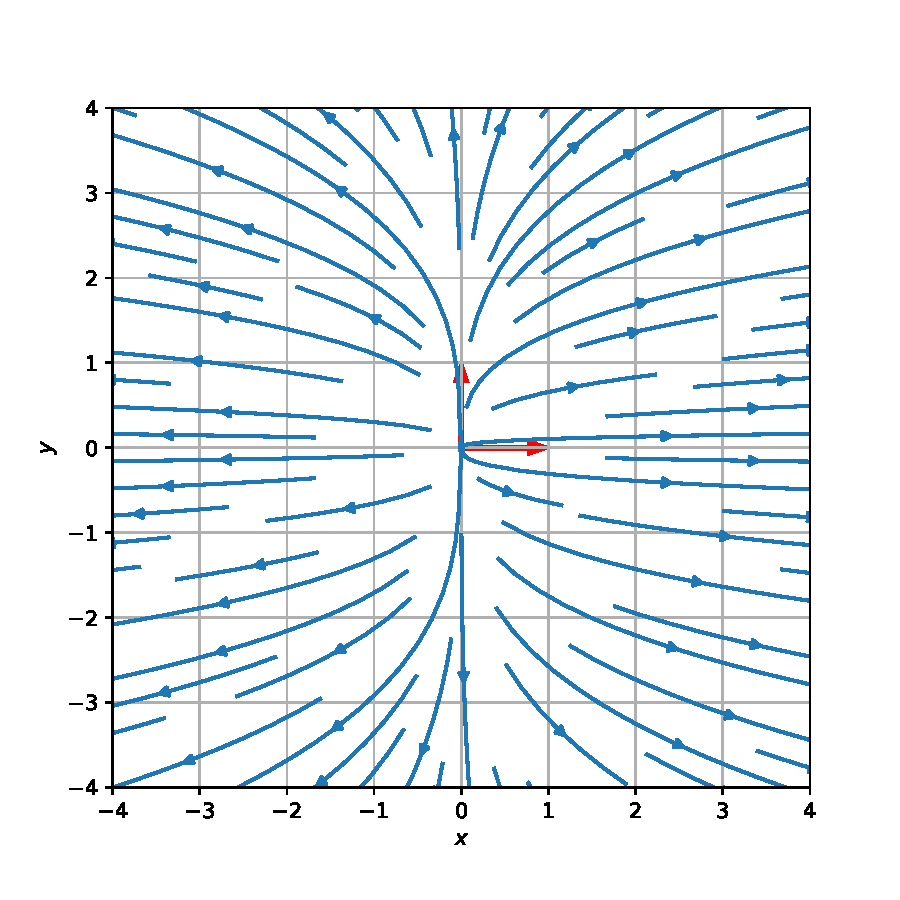
\includegraphics[scale=0.55]{1a1_0}
	\caption{Фазовый портрет в канонических координатах}
	\label{im:1a1_0}
\end{figure}



(iv) Фазовый портрет(\ref{eq:1}) в исходных координатах:

\begin{figure}[H]
	\centering
	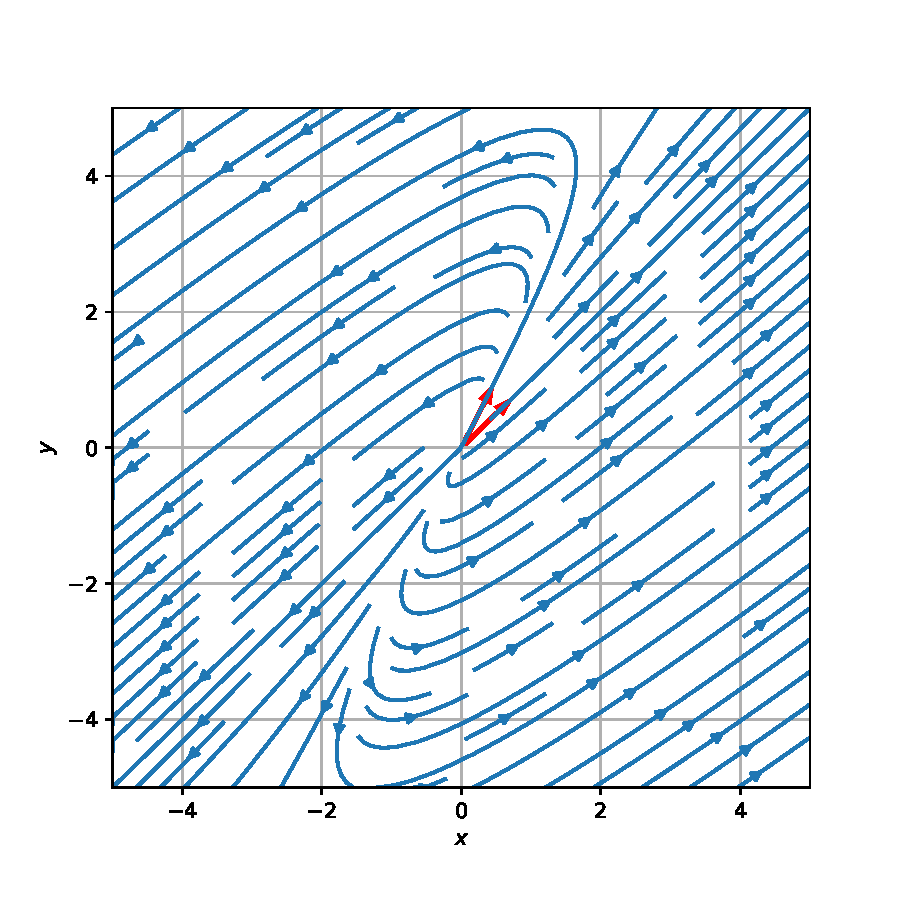
\includegraphics[scale=0.55]{1a1_1}
	\caption{Фазовый портрет в исходных координатах}
	\label{im:1a1_1}
\end{figure}

(v) $\lambda_{1,2}>0$, картина -- \textbf{неустойчивый узел}.


	\subsection* {Задача 2}
 Решить систему дифференциальных уравнений (Задача Коши): 
\begin{equation}
\left\{
\begin{array}{lr}
\dot{x} = x+2y+2e^{-t}\\
\dot{y} = 2x+y
\end{array}
\right.
, \;\;\;\; x(\cdot)\in \textbf{R},\; y(\cdot)\in \textbf{R}
\label{eq:16}
\end{equation}

\textbf{Решение:} \par


(i) Найти общее решение соответствующей однородной системы.\\
Собственные векторы и собственные значения для матрицы однородного уравнения:
\[\lambda_1 = 3:\;\;\;\;\; p^1=
\left(
\begin{array}{cc}
1\\
1\\
\end{array}
\right)  
\]

\[\lambda_2=-1\;\;\;\; p^2=
\left(
\begin{array}{cc}
-1\\
1\\
\end{array}
\right) 
\]
Общее решение:
\[\left(
\begin{array}{c}
x(t)\\
y(t)
\end{array}
\right)=C_1\left(
\begin{array}{c}
1 \\
1
\end{array}
\right)e^{3t}+C_2\left(
\begin{array}{c}
-1 \\
1
\end{array}
\right)e^{-t}\]
Частное решение будем искать методом вариации постоянной:
\[\left(
\begin{array}{c}
x(t)\\
y(t)
\end{array}
\right)=C_1(t)\left(
\begin{array}{c}
1 \\
1
\end{array}
\right)e^{3t}+C_2(t)\left(
\begin{array}{c}
-1 \\
1
\end{array}
\right)e^{-t}\]
Подставляя эти выражения в систему (\ref{eq:16}), получим:

\[
\left\{
\begin{array}{lr}
C_1  = - \frac 1 4 e^{-4t}\\
C_2 = t
\end{array}
\right.
\]
Общее решение уравнения есть сумма частного и однородного:

\begin{equation}
x(t) = C_1e^{3t}-C_2e^{-t}-e^{-t}\left(\frac 1 4 + t\right)
\label{eq:17}
\end{equation}
\begin{equation}
y(t) = C_1e^{3t}+C_2e^{-t}+e^{-t}\left(t-\frac 1 4 \right)
\label{eq:18}
\end{equation}

(ii) Найти траекторию системы (\ref{eq:16}), проходящую через начало координат.\\
Подставляя точку $(0;0;0)$ в (\ref{eq:17}) и (\ref{eq:18}), находим константы $C_1$ и $C_2$:

\[C_1 = \frac 1 4 \;\;\;\;\; C_2 =0\]

\[
x_0(t) =\frac 1 4\left(e^{3t} -4te^{-t}-e^{-t}\right)\]
\[
y_0(t) = \frac 1 4\left(e^{3t} +4te^{-t}-e^{-t}\right)
\]

(iii) Для траектории, найденной в (ii), найти пределы $\lim_{t\rightarrow\pm\infty}y(t)/x(t)$ (если они существуют).


\[\lim_{t\rightarrow+\infty}\frac{\frac 1 4\left(e^{3t} -4te^{-t}-e^{-t}\right)}{ \frac 1 4\left(e^{3t} +4te^{-t}-e^{-t}\right)}=1 \]

\[\lim_{t\rightarrow-\infty}\frac{\frac 1 4\left(e^{3t} -4te^{-t}-e^{-t}\right)}{ \frac 1 4\left(e^{3t} +4te^{-t}-e^{-t}\right)}=-1\]


	\subsection* {Задача 3}
Для дифференциального уравнения 
\begin{equation}
y''+4y'+4y=\frac {e^{-2x}}{2x^2}, \;\;\;\; y(\cdot)\in \textbf{R},\; x>0
\label{eq:5}
\end{equation}

(i) Найти общее решение соотвествующего однородного уравнения.\\
\[y(x) = e^{ax}\]
\[a^2+4a+4=0\]
\[a = -2\]
Тогда решение:
\[y(x)=C_1e^{-2x}+C_2xe^{-2x}\]

(ii) Найти общее решение уравнения (\ref{eq:5}).\\
Будем решать уравнение методом вариации постоянной:

\[y(x)= C_1(x)e^{-2x}+C_2(x)xe^{-2x}\]
Получим систему:
\[ \left(
\begin{array}{cc}
e^{-2x} & xe^{-2x} \\
-2e^{-2x} & e^{-2x}(1-2x)
\end{array}
\right) \left(
\begin{array}{c}
C_1' \\
C_2'
\end{array} 
\right)= \left(
\begin{array}{c}
0 \\
e^{-2x}/2x^2
\end{array}
\right) \]
Найдем коэффициенты:
\[C_1' = -\frac 1 {2x}\]

\[C_2' = \frac 1  {2x^2}\]
Тогда общее решение:
\[y(x) = C_1e^{-2x}+C_2xe^{-2x}-\frac 1 2 e^{-2x}\ln(x)\]




	\subsection* {Задача 4}

Для дифференциального уравнения
\begin{equation}
y''+y'-2y=3xe^x, \;\;\;\; y(\cdot)\in \textbf{R}, \; x(\cdot)\in \textbf{R}
\label{eq:6}
\end{equation}

(i) найти общее решение соответствующего однородного уравнения.\\
Характеристическое уравнение для левой части (\ref{eq:6}):
\[a^2+a-2=0\]
\[a_{1}=1,\;\;\;\; a_2 = -2\]
Тогда общее решение однородного уравнения:
\begin{equation}
y(x) = C_1e^{-2x}+C_2e^x
\label{eq:7}
\end{equation}

(ii) найти общее решение уравнения (\ref{eq:6}).\\
Частное решение для этой правой части ищем в виде:
\[ y_{\text{частн}} = (Ax+B)xe^x\]
Поставляя в (\ref{eq:6}), находим коэффициенты: 
\[
\left\{
\begin{array}{lr}
B = -\frac 1 3 \\
A = \frac 1 2
\end{array}
\right.
\]
Суммируя частное и однородное решения, получим ответ:

\[y(x) = C_1e^{-2x}+C_2e^x+\frac{e^xx^2}{2}-\frac{e^xx}{3} \]


	\section*{Вариант II}
		\subsection* {Задача 1}


 Решить систему дифференциальных уравнений (Задача Коши): 
\begin{equation}
\left\{
\begin{array}{lr}
\dot{x} = 7x+3y\\
\dot{y} = x-y
\end{array}
\right.
, \;\;\;\; x(\cdot)\in \textbf{R},\; y(\cdot)\in \textbf{R}
\label{eq:1}
\end{equation}

\textbf{Решение:} \par
Обозначим 
\[
A = \left(
\begin{array}{cc}
7 & 3\\
1 & -1\\
\end{array}
\right)\]

(i) Стационарные точки:

\[
\left\{
\begin{array}{lr}
\dot{x} = 0\\
\dot{y} = 0
\end{array}
\right.
\Leftrightarrow (0;0)
\]


(ii) Найдем собственные числа матрицы A:
\[det(A-\lambda \hat{I})=
\begin{vmatrix}
7-\lambda & 3 \\
1 & -1-\lambda
\end{vmatrix}
=0\]

\[\lambda_1=3+\sqrt{19}, \; \lambda_2=3-\sqrt{19}\]
\\Найдем собственные векторы:
\[\lambda_1=3+\sqrt{19},\;\;\;\;\; p^1=
\left(
\begin{array}{cc}
4+\sqrt{19}\\
1\\
\end{array}
\right)
\]



\[\lambda_2=3-\sqrt{19},\;\;\;\; p^2=
\left(
\begin{array}{cc}
4-\sqrt{19}\\
1\\
\end{array}
\right)
\]
Каноническое преобразование координат:
\[A = S\Lambda S^{-1}\]
\[
S = \left(
\begin{array}{cc}
4-\sqrt{19} & 4+\sqrt{19}\\
1 & 1\\
\end{array}
\right)\;\;\;\;\;
S^{-1} = \left(
\begin{array}{cc}
-\frac{1}{2\sqrt{19}} & \frac 1 2 +\frac{2}{\sqrt{19}}\\
\frac{1}{2\sqrt{19}} & \frac 1 2 -\frac{2}{\sqrt{19}}\\
\end{array}\right)\;\;\;\;\;
\Lambda = \left(
\begin{array}{cc}
3-\sqrt{19} & 0\\
0 & 3+\sqrt{19}\\
\end{array}\right)
\]

Система в новых координатах:
\[\left(
\begin{array}{c}
\dot{\alpha}_1\\
\dot{\alpha}_2
\end{array}
\right)=\Lambda\left(
\begin{array}{c}
{\alpha}_1 \\
{\alpha}_2
\end{array}
\right)\]


(iii) Прямые, при пересечении которых фазовые траектории параллельны осям $x$ и $y$.\\
Параллельно оси y:
\[\dot{x} = 7x+3y=0\Leftrightarrow y = -7/3x\]\\
Параллельно оси x:
\[\dot{y} = x-y=0\Leftrightarrow y = x\]
\begin{figure}[H]
	\centering
	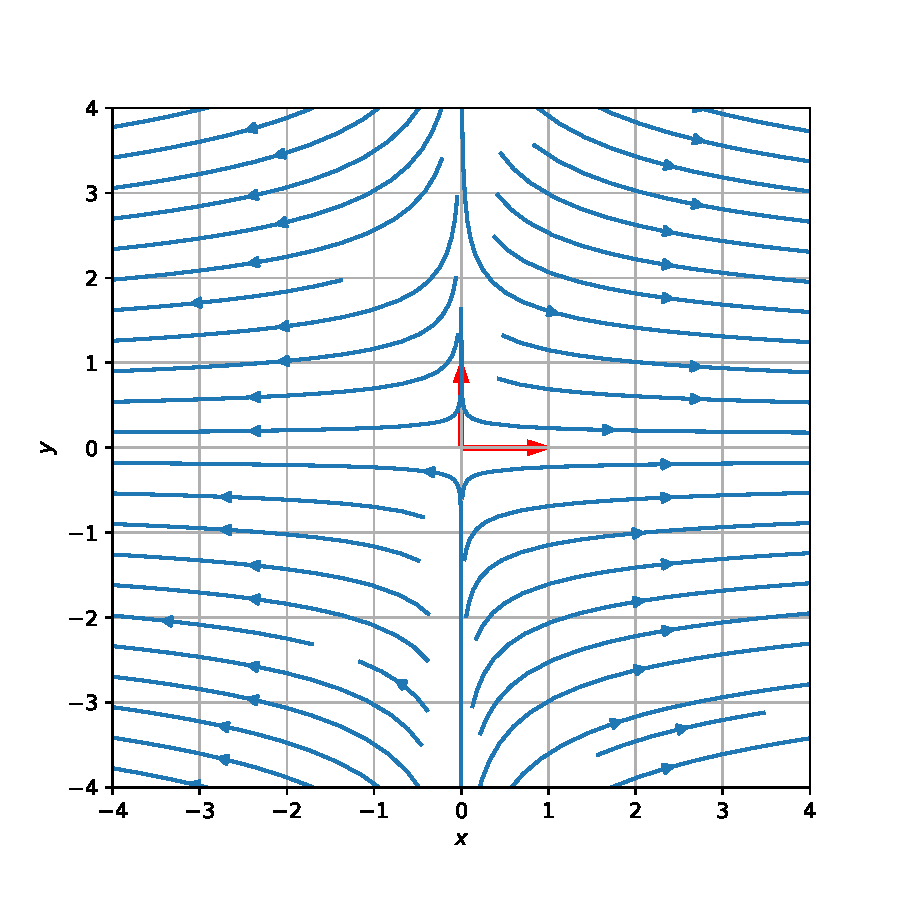
\includegraphics[scale=0.8]{2a1_0}
	\caption{Фазовый портрет в канонических координатах}
	\label{im:2a1_0}
\end{figure}



(iv) Фазовый портрет(\ref{eq:1}) в исходных координатах:

\begin{figure}[H]
	\centering
	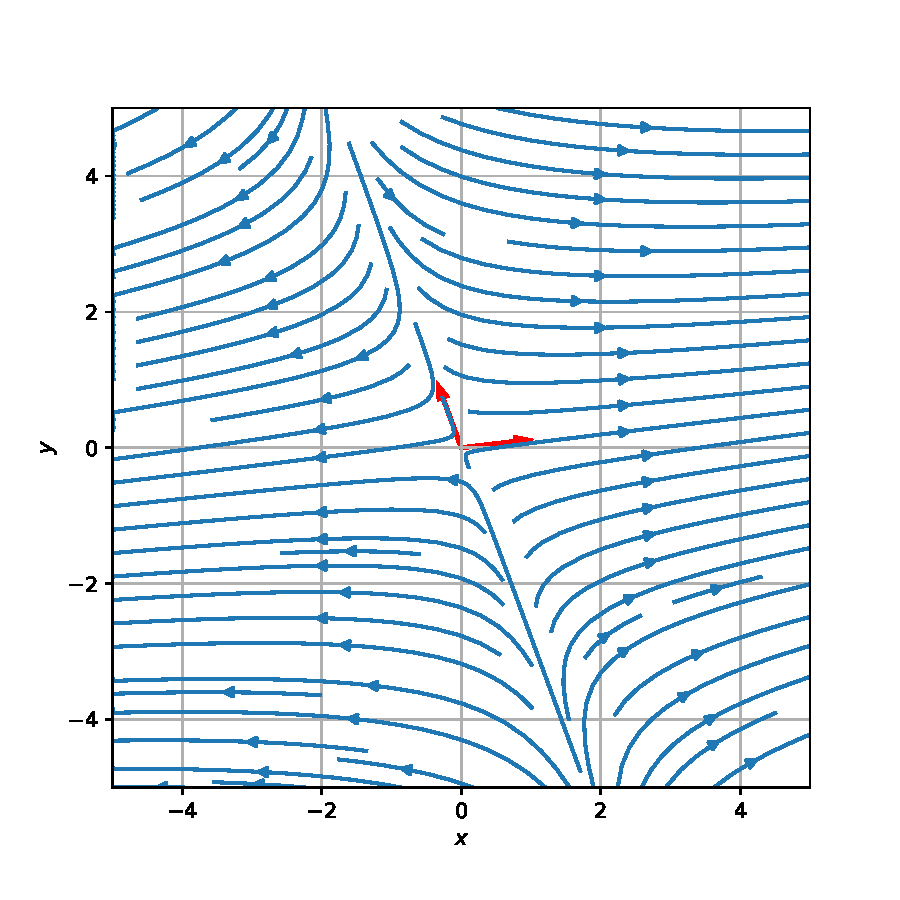
\includegraphics[scale=0.7]{2a1_1}
	\caption{Фазовый портрет в исходных координатах}
	\label{im:2a1_1}
\end{figure}

(v) $\lambda_{1,2}$ разных знаков, картина -- \textbf{седло}.


	\subsection* {Задача 2}
 Решить систему дифференциальных уравнений (Задача Коши): 
\begin{equation}
\left\{
\begin{array}{lr}
\dot{x} = -x+4y+e^{-t}\\
\dot{y} = 2x+y+1
\end{array}
\right.
, \;\;\;\; x(\cdot)\in \textbf{R},\; y(\cdot)\in \textbf{R}
\label{eq:23}
\end{equation}

\textbf{Решение:} \par


(i) Найти общее решение соответствующей однородной системы.\\

Собственные векторы и собственные значения для матрицы однородного уравнения:
\[\lambda_1 = -3:\;\;\;\;\; p^1=
\left(
\begin{array}{cc}
-2\\
1\\
\end{array}
\right)  
\]



\[\lambda_2=3\;\;\;\; p^2=
\left(
\begin{array}{cc}
1\\
1\\
\end{array}
\right) 
\]

Общее решение:
\[\left(
\begin{array}{c}
x(t)\\
y(t)
\end{array}
\right)=C_1\left(
\begin{array}{c}
-2 \\
1
\end{array}
\right)e^{-3t}+C_2\left(
\begin{array}{c}
1 \\
1
\end{array}
\right)e^{3t}\]

Частное решение будем искать в следующем виде:
\[x(t)_{\text{частн}}=a+be^{-t}\]
\[y(t)_{\text{частн}}=c+de^{-t}\]
Подставляя эти выражения в систему (\ref{eq:23}), получим:

\[
\left\{
\begin{array}{lr}
a = -\frac {4} {9}\\
b = \frac {1} {4}\\
c = -\frac {1} {9}\\
d = -\frac {1} {4}\\
\end{array}
\right.
\]
Общее решение уравнения есть сумма частного и однородного:

\begin{equation}
x(t) = -2C_1e^{-3t}+C_2e^{3t}-\frac 4 9 + \frac 1 4 e^{-t}
\label{eq:24}
\end{equation}
\begin{equation}
y(t) =C_1e^{-3t}+C_2e^{3t}- \frac 1 9 -\frac 1 4 e^{-t}
\label{eq:25}
\end{equation}

(ii) Найти траекторию системы (\ref{eq:23}), проходящую через начало координат.\\
Подставляя точку $(0;0;0)$ в (\ref{eq:24}) и (\ref{eq:24}), находим константы $C_1$ и $C_2$:

\[C_1 = \frac 1 {18}\;\;\;\;\; C_2 = \frac{11} {36}\]

\[
x_0(t) =-\frac 1 9 e^{-3t}+\frac{11}{36}e^{3t}-\frac 4 9 + \frac 1 4 e^{-t}\]
\[
y_0(t) =\frac 1 {18}e^{-3t}+\frac{11} {36} e^{3t}- \frac 1 9 -\frac 1 4 e^{-t}
\]

(iii) Для траектории, найденной в (ii), найти пределы $\lim_{t\rightarrow\pm\infty}y(t)/x(t)$ (если они существуют).


\[\lim_{t\rightarrow+\infty}\frac{\frac 1 {18}e^{-3t}+\frac{11} {36} e^{3t}- \frac 1 9 -\frac 1 4 e^{-t}}{-\frac 1 9 e^{-3t}+\frac{11}{36}e^{3t}-\frac 4 9 + \frac 1 4 e^{-t}}= 1\]

\[\lim_{t\rightarrow-\infty}\frac{\frac 1 {18}e^{-3t}+\frac{11} {36} e^{3t}- \frac 1 9 -\frac 1 4 e^{-t}}{-\frac 1 9 e^{-3t}+\frac{11}{36}e^{3t}-\frac 4 9 + \frac 1 4 e^{-t}}=-\frac 1 2\]

	\subsection*{Задача 3}
Для дифференциального уравнения 
\begin{equation}
y''+3y'+2y=\frac {1}{e^x+1}, \;\;\;\; y(\cdot)\in \textbf{R},\; x(\cdot)\in \textbf{R}
\label{eq:2_3}
\end{equation}

(i) Найти общее решение соотвествующего однородного уравнения.\\
\[y(x) = e^{ax}\]
\[a^2+3a+2=0\]
\[a_1 = -1,\;\; a_2 = -2\]
Тогда решение:
\[y(x)=C_1e^{-x}+C_2e^{-2x}\]

(ii) Найти общее решение уравнения (\ref{eq:2_3}).\\
Будем решать уравнение методом вариации постоянной:

\[y(x)= C_1(x)e^{-x}+C_2(x)e^{-2x}\]
Получим систему:
\[ \left(
\begin{array}{cc}
e^{-x} & e^{-2x} \\
-e^{-x} & -2e^{-2x}
\end{array}
\right) \left(
\begin{array}{c}
C_1' \\
C_2'
\end{array} 
\right)= \left(
\begin{array}{c}
0 \\
\frac {1}{e^x+1}
\end{array}
\right) \]
Найдем коэффициенты:
\[C_1 = \ln (e^x+1)\]
\[C_2 = \ln (e^x+1)-e^x\]
Тогда общее решение:
\[y(x)= C_1(x)e^{-x}+C_2(x)e^{-2x}+e^{-x} \ln (e^x+1)+e^{-2x}\ln (e^x+1)\]




	\subsection* {Задача 4}

Для дифференциального уравнения
\begin{equation}
y''-5y'+4y=4x^2e^{2x}, \;\;\;\; y(\cdot)\in \textbf{R}, \; x(\cdot)\in \textbf{R}
\label{eq:2_4}
\end{equation}

(i) найти общее решение соответствующего однородного уравнения.\\
Характеристическое уравнение для левой части (\ref{eq:2_4}):
\[a^2-5a+4=0\]
\[a_{1}=1,\;\;\;\; a_2 = 4\]
Тогда общее решение однородного уравнения:
\begin{equation}
y(x) = C_1e^{x}+C_2e^{4x}
\label{eq:7}
\end{equation}

(ii) найти общее решение уравнения (\ref{eq:2_4}).\\
Частное решение для этой правой части ищем в виде:
\[ y_{\text{частн}} = Ae^{2x}+Bxe^{2x}+Cx^2e^{2x}\]
Поставляя в (\ref{eq:2_4}), находим коэффициенты: 
\[
\left\{
\begin{array}{lr}
A = -3 \\
B  = 2\\
C = -2
\end{array}
\right.
\]
Суммируя частное и однородное решения, получим ответ:

\[y(x) = C_1e^{x}+C_2e^{4x}-3e^{2x} +2xe^{2x} -2x^2e^{2x} \]




	\section*{Вариант III}
		\subsection* {Задача 1}


 Решить систему дифференциальных уравнений (Задача Коши): 
\begin{equation}
\left\{
\begin{array}{lr}
\dot{x} = 2x+7y\\
\dot{y} = -2x-2y
\end{array}
\right.
, \;\;\;\; x(\cdot)\in \textbf{R},\; y(\cdot)\in \textbf{R}
\label{eq:1}
\end{equation}

\textbf{Решение:} \par
Обозначим 
\[
A = \left(
\begin{array}{cc}
2 & 7\\
-2 & -2\\
\end{array}
\right)\]

(i) Стационарные точки:

\[
\left\{
\begin{array}{lr}
\dot{x} = 0\\
\dot{y} = 0
\end{array}
\right.
\Leftrightarrow (0;0)
\]


(ii) Найдем собственные числа матрицы A:
\[det(A-\lambda \hat{I})=
\begin{vmatrix}
2-\lambda & 7 \\
-2 & -2-\lambda
\end{vmatrix}
=0\]

\[\lambda_1=-i\sqrt{10}, \; \lambda_2=i\sqrt{10}\]
\\Найдем собственные векторы:
\[\lambda_1=i\sqrt{10},\;\;\;\;\; p^1=
\left(
\begin{array}{cc}
\frac 1 2 (-2-i\sqrt{10})\\
1\\
\end{array}
\right)=\left(
\begin{array}{cc}
-1\\
1\\
\end{array}
\right) +i
\left(
\begin{array}{cc}
-\frac{\sqrt{10}}{2}\\
0\\
\end{array}
\right)
\]



\[\lambda_2=-i\sqrt{10},\;\;\;\; p^2=
\left(
\begin{array}{cc}
\frac 1 2 (-2+i\sqrt{10})\\
1\\
\end{array}
\right) 
\]

Каноническое преобразование координат:
\[A = S\Lambda S^{-1}\]
\[
S = \left(
\begin{array}{cc}
-1& \frac{\sqrt{10}}{2}\\
1 & 0\\
\end{array}
\right)\;\;\;\;\;
S^{-1} = \left(
\begin{array}{cc}
0 & 1\\
\sqrt{\frac {2}{5}} & \sqrt{\frac {2}{5}}\\
\end{array}\right)\;\;\;\;\;
\Lambda = \left(
\begin{array}{cc}
0 & -\sqrt{10}\\
\sqrt{10} & 0\\
\end{array}\right)
\]

Система в новых координатах:
\[\left(
\begin{array}{c}
\dot{\alpha}_1\\
\dot{\alpha}_2
\end{array}
\right)=\Lambda\left(
\begin{array}{c}
{\alpha}_1 \\
{\alpha}_2
\end{array}
\right)\]


(iii) Прямые, при пересечении которых фазовые траектории параллельны осям $x$ и $y$.\\
Параллельно оси y:
\[\dot{x} = 2x+7y=0\Leftrightarrow y = -2/7x\]\\
Параллельно оси x:
\[\dot{y} = -2x-y=0\Leftrightarrow y = -x\]
\begin{figure}[H]
	\centering
	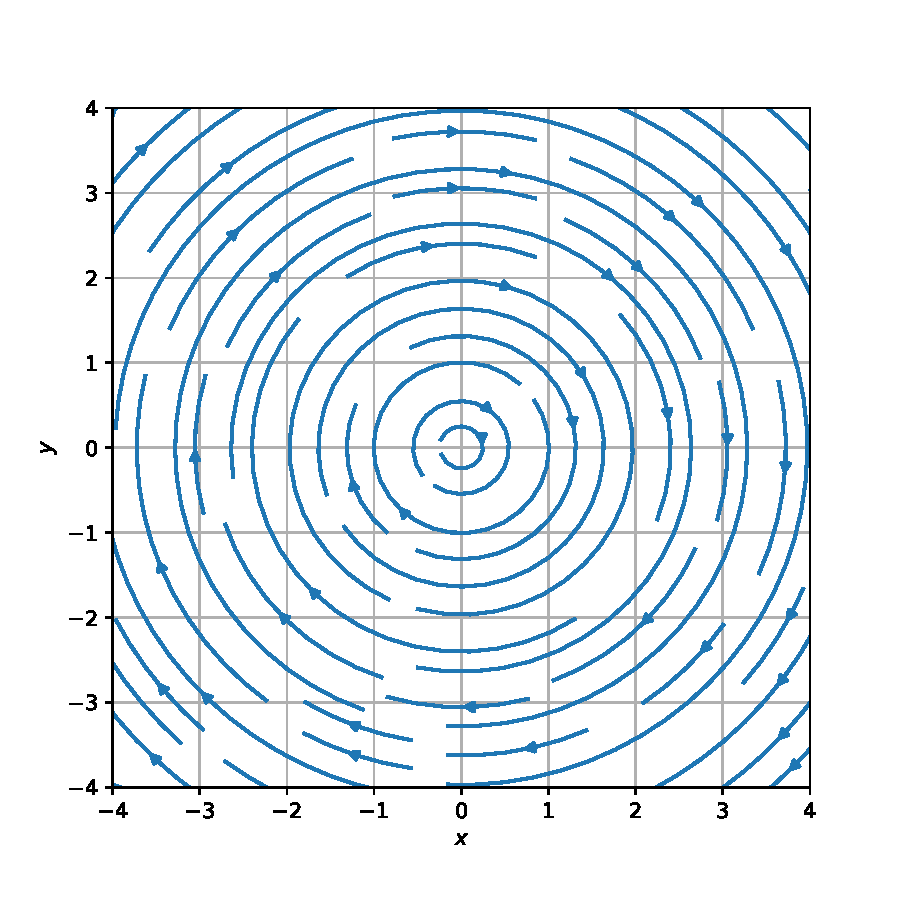
\includegraphics[scale=0.7]{3a1_0}
	\caption{Фазовый портрет в канонических координатах}
	\label{im:3a1_0}
\end{figure}



(iv) Фазовый портрет(\ref{eq:1}) в исходных координатах:

\begin{figure}[H]
	\centering
	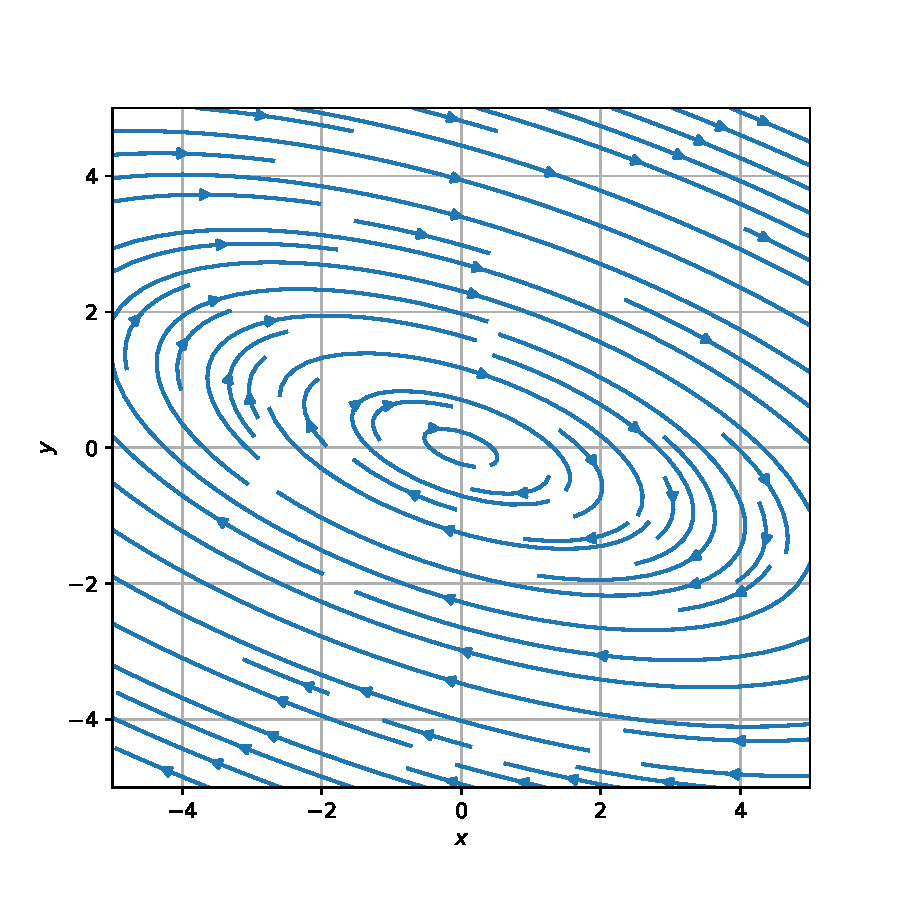
\includegraphics[scale=0.7]{3a1_1}
	\caption{Фазовый портрет в исходных координатах}
	\label{im:3a1_1}
\end{figure}

(v) $Re(\lambda_{1,2})=0$, картина -- \textbf{центр}.






	\subsection* {Задача 2}
 Решить систему дифференциальных уравнений (Задача Коши): 
\begin{equation}
\left\{
\begin{array}{lr}
\dot{x} = -x+4y+\sin{t}\\
\dot{y} = 2x-y
\end{array}
\right.
, \;\;\;\; x(\cdot)\in \textbf{R},\; y(\cdot)\in \textbf{R}
\label{eq:30}
\end{equation}

\textbf{Решение:} \par


(i) Найти общее решение соответствующей однородной системы.\\

Собственные векторы и собственные значения для матрицы однородного уравнения:
\[\lambda_1 = -1-2\sqrt 2 :\;\;\;\;\; p^1=
\left(
\begin{array}{cc}
-\sqrt 2\\
1\\
\end{array}
\right)  
\]



\[\lambda_2=2\sqrt 2-1\;\;\;\; p^2=
\left(
\begin{array}{cc}
\sqrt 2\\
1\\
\end{array}
\right) 
\]

Общее решение:
\[\left(
\begin{array}{c}
x(t)\\
y(t)
\end{array}
\right)=C_1\left(
\begin{array}{c}
-\sqrt 2 \\
1
\end{array}
\right)e^{(-1-2\sqrt 2)t}+C_2\left(
\begin{array}{c}
\sqrt 2 \\
1
\end{array}
\right)e^{(2\sqrt 2-1)t}\]

Частное решение будем искать в следующем виде:
\[x(t)_{\text{частн}}=a\cos{t}+b\sin{t}\]
\[y(t)_{\text{частн}}=c\cos{t}+d\sin{t}\]
Подставляя эти выражения в систему (\ref{eq:30}), получим:

\[
\left\{
\begin{array}{lr}
a = -\frac {5} {34}\\
b = -\frac {3} {34}\\
c = -\frac {1} {17}\\
d = -\frac {4} {17}\\
\end{array}
\right.
\]
Общее решение уравнения есть сумма частного и однородного:

\begin{equation}
x(t) = -C_1\sqrt 2 e^{(-1-2\sqrt 2)t}+C_2\sqrt 2 e^{(-1+2\sqrt 2)t} -\frac {5} {34}\cos{t}-\frac {3} {34}\sin{t}
\label{eq:31}
\end{equation}
\begin{equation}
y(t) =C_1 e^{(-1-2\sqrt 2)t}+C_2 e^{(-1+2\sqrt 2)t} -\frac {1} {17}\cos{t}-\frac {4} {17}\sin{t}
\label{eq:32}
\end{equation}

(ii) Найти траекторию системы (\ref{eq:30}), проходящую через начало координат.\\
Подставляя точку $(0;0;0)$ в (\ref{eq:31}) и (\ref{eq:32}), находим константы $C_1$ и $C_2$:

\[C_1 = \frac{5\sqrt{2}-4}{136}\;\;\;\;\; C_2 = \frac{12- 5\sqrt{2}}{136}\]

\[
x_0(t) = -\frac{5-2\sqrt{2}}{68} e^{(-1-2\sqrt 2)t}+\frac{6\sqrt{2}- 5}{68} e^{(-1+2\sqrt 2)t} -\frac {5} {34}\cos{t}-\frac {3} {34}\sin{t}
\]\[
y_0(t) = \frac{5\sqrt{2}-4}{136} e^{(-1-2\sqrt 2)t}+\frac{12- 5\sqrt{2}}{136}e^{(-1+2\sqrt 2)t} -\frac {1} {17}\cos{t}-\frac {4} {17}\sin{t}
\]

(iii) Для траектории, найденной в (ii), найти пределы $\lim_{t\rightarrow\pm\infty}y(t)/x(t)$ (если они существуют).


\[\lim_{t\rightarrow+\infty}\frac{\frac{5\sqrt{2}-4}{136} e^{(-1-2\sqrt 2)t}+\frac{12- 5\sqrt{2}}{136}e^{(-1+2\sqrt 2)t} -\frac {1} {17}\cos{t}-\frac {4} {17}\sin{t}}{-\frac{5-2\sqrt{2}}{68} e^{(-1-2\sqrt 2)t}+\frac{6\sqrt{2}- 5}{68} e^{(-1+2\sqrt 2)t} -\frac {5} {34}\cos{t}-\frac {3} {34}\sin{t}}=\frac {1} {\sqrt2} \]

\[\lim_{t\rightarrow-\infty}\frac{\frac{5\sqrt{2}-4}{136} e^{(-1-2\sqrt 2)t}+\frac{12- 5\sqrt{2}}{136}e^{(-1+2\sqrt 2)t} -\frac {1} {17}\cos{t}-\frac {4} {17}\sin{t}}{-\frac{5-2\sqrt{2}}{68} e^{(-1-2\sqrt 2)t}+\frac{6\sqrt{2}- 5}{68} e^{(-1+2\sqrt 2)t} -\frac {5} {34}\cos{t}-\frac {3} {34}\sin{t}}=-\frac {1} {\sqrt2}\]

	\subsection*{Задача 3}
Для дифференциального уравнения 
\begin{equation}
y''+y=\frac {1}{\sin x}, \;\;\;\; y(\cdot)\in \textbf{R},\; x\in (0,\pi/2)
\label{eq:3_3}
\end{equation}

(i) Найти общее решение соотвествующего однородного уравнения.\\
Левая часть (\ref{eq:3_3}) -- уравнение осциллятора. Его решение:
\[y(x)=C_1e^{ix}+C_2e^{-ix}=C_1\cos x+C_2\sin x\]

(ii) Найти общее решение уравнения (\ref{eq:3_3}).\\
Будем решать уравнение методом вариации постоянной:

\[y(x)= C_1(x)\cos x+C_2(x)\sin x\]
Получим систему:
\[ \left(
\begin{array}{cc}
\cos x & \sin x \\
-\sin x & \cos x
\end{array}
\right) \left(
\begin{array}{c}
C_1' \\
C_2'
\end{array} 
\right)= \left(
\begin{array}{c}
0 \\
\frac {1}{\sin x}
\end{array}
\right) \]
Найдем коэффициенты: 
\[C_1=-x\]
\[C_2=\ln(\sin x)\]
Тогда общее решение:
\[y(x)= C_1(x)\cos x+C_2(x)\sin x-x\cos x+\ln(\sin x)\sin x\]



	\subsection* {Задача 4}

Для дифференциального уравнения
\begin{equation}
y''+y=4xe^x, \;\;\;\; y(\cdot)\in \textbf{R}, \; x(\cdot)\in \textbf{R}
\label{eq:3_4}
\end{equation}

(i) найти общее решение соответствующего однородного уравнения.\\
Левая часть (\ref{eq:3_4}) -- уравнение осциллятора:
\begin{equation}
y(x) = C_1e^{-ix}+C_2e^{+ix} = C_1\sin{x}+C_2\cos{x}
\label{eq:3_4}
\end{equation}

(ii) найти общее решение уравнения (\ref{eq:3_4}).\\
Частное решение для этой правой части ищем в виде:
\[ y_{\text{частн}} = Ae^{x}+Bxe^{x}\]
Поставляя в (\ref{eq:3_4}), находим коэффициенты: 
\[
\left\{
\begin{array}{lr}
A = -2 \\
B  = 2
\end{array}
\right.
\]
Суммируя частное и однородное решения, получим ответ:

\[y(x) =C_1\sin{x}+C_2\cos{x}-2e^x+2xe^x\]





\end{document}